% ctex_test.tex
\documentclass{article}

% Language setting
% Replace `english' with e.g. `spanish' to change the document language
\usepackage[UTF8]{ctex}
\usepackage{setspace}
\usepackage{listings}
\usepackage{xcolor}
\usepackage[colorlinks,linkcolor=blue]{hyperref}
\usepackage{enumitem}
\usepackage{tabularx}
\usepackage{longtable}
\usepackage{makecell}
\usepackage{multirow}
\usepackage{array}
\renewcommand\theadfont{\bfseries}
\renewcommand\theadgape{}

\lstset{
  backgroundcolor=\color{white},
  basicstyle=\ttfamily\footnotesize,
  breakatwhitespace=false,
  breaklines=true,
  captionpos=b,
  commentstyle=\color{mygreen},
  deletekeywords={...},
  escapeinside={\%*}{*)},
  frame=single,
  keepspaces=true,
  keywordstyle=\color{blue},
  language=Python,
  morekeywords={*,...},
  numbers=left,
  numbersep=5pt,
  numberstyle=\tiny\color{mygray},
  rulecolor=\color{black},
  showspaces=false,
  showstringspaces=false,
  showtabs=false,
  stepnumber=2,
  stringstyle=\color{mymauve},
  tabsize=2,
  title=\lstname
}


% Set page size and margins
% Replace `letterpaper' with `a4paper' for UK/EU standard size
\usepackage[letterpaper,top=2cm,bottom=2cm,left=3cm,right=3cm,marginparwidth=1.75cm]{geometry}

% Useful packages
\usepackage{amsmath}
\usepackage{graphicx}
\usepackage[colorlinks=true, allcolors=blue]{hyperref}

\title{当代人工智能实验报告4}
\author{温兆和 10205501432}

\begin{document}
\maketitle

\section{实验目的}
在本次实验中,我们使用PyTorch工具构建并训练了多个不同的循环神经网络,使得模型能够根据输入的病情描述生成相应的诊断。

\section{实验环境}
出于实际需要,本次实验是在autodl上租来的云实例上进行的。

\textbf{云实例的具体配置情况:}
\begin{spacing}{0.5}
\begin{itemize}
\item 镜像:
    \begin{itemize}
        \item PyTorch 2.0.0
        \item Python 3.8(ubuntu 20.04)
        \item Cuda 11.8
    \end{itemize} 
\item GPU:RTX 4090(24GB) * 1 
\item CPU:22 vCPU AMD EPYC 7T83 64-Core Processor
\item 内存:90GB
\item 硬盘:
    \begin{itemize}
        \item 系统盘:30 GB
        \item 数据盘:
            \begin{itemize}
                \item 免费:50GB
                \item 付费:0GB
            \end{itemize}
    \end{itemize}
\item 附加磁盘:无
\item 端口映射:无
\item 网络:同一地区实例共享带宽
\end{itemize}
\end{spacing}

\textbf{需要安装的工具包有:}
\begin{spacing}{0.5}
\begin{itemize}
\item \lstinline|numpy|
\item \lstinline|torch|
\item \lstinline|pandas|
\item \lstinline|rouge_score|
\item \lstinline|tensorflow|
\item \lstinline|tensorflow_intel|
\item \lstinline|matplotlib|
\end{itemize}
\end{spacing}

如果需要安装这些包,可以在项目路径下执行\lstinline|pip install -r requirements.txt|命令。
\section{实验步骤}
\subsection{数据预处理}
在自然语言处理中,数据预处理是个大问题,因为文本数据并不像图像数据那样天然地可以用张量来表示,需要通过一定的手段把它转化为张量。此外,在本次实验中,为了保护病人的隐私,本次实验的文本数据都经过了脱敏,数据集中的“文本”实际上是由多个数字组成的字符串,它们的长度还各不相同。起初,我以为这是文本已经被转化为张量,只需要把这些张量padding到同一个长度并输入到模型中去训练就好了。但后来我发现,无论是BLEU,ROUGE还是CIDEr,都是需要把文本(而不是张量)作为输入去计算相应指标的得分的。于是我询问助教应该怎么处理这种情况,助教告诉我直接把数据集中的“张量”当成文本去处理就好了。

具体来说,在训练开始前,在数据集上拟合一个tokenizer,并用tokenizer把所有的“文本”(其实就是张量)转化为向量:
\begin{lstlisting}
from tensorflow.keras.preprocessing.text import Tokenizer

train_and_valid = pd.read_csv('./train.csv')
test = pd.read_csv('./test.csv')
combined_data = pd.concat([train_and_valid, test])
combined_texts = combined_data['description'] + ' ' + combined_data['diagnosis']
text_tokenizer = Tokenizer(num_words=vocab_size, oov_token='<OOV>')
text_tokenizer.fit_on_texts(combined_texts)
train_desc_seq = text_tokenizer.texts_to_sequences(train_and_valid['description'])
train_diag_seq = text_tokenizer.texts_to_sequences(train_and_valid['diagnosis'])
test_desc_seq = text_tokenizer.texts_to_sequences(test['description'])
test_diag_seq = text_tokenizer.texts_to_sequences(test['diagnosis'])
\end{lstlisting}
把所有这些向量都填补到同一个长度,就得到了可以用来训练模型的数据:
\begin{lstlisting}
from tensorflow.keras.preprocessing.sequence import pad_sequences

train_desc_seq = pad_sequences(train_desc_seq, maxlen=max_len, padding='post')
train_diag_seq = pad_sequences(train_diag_seq, maxlen=max_len, padding='post')
test_desc_seq = pad_sequences(test_desc_seq, maxlen=max_len, padding='post')
test_diag_seq = pad_sequences(test_diag_seq, maxlen=max_len, padding='post')
\end{lstlisting}
在评估模型的输出时,我们还得把输出从向量转化为文本(其实还会是一个个的数字),才能计算那些用以评估模型的指标:
\begin{lstlisting}
def sequence_to_text(sequence, tokenizer):
    reverse_word_index = {index: word for word, index in tokenizer.word_index.items()}
    output_text = ' '.join([reverse_word_index.get(i, '') for i in sequence])
    if len(output_text) == 1:
        output_text = output_text.join('<OOV>')
    return output_text
……
output_text = sequence_to_text(output,text_tokenizer)
\end{lstlisting}

\subsection{模型原理与构建}
\subsubsection{普通RNN}
RNN本质上是一种专门设计用于处理序列数据的神经网络结构,其基本思想是在处理序列数据时引入循环结构,以便模型可以记忆先前的信息并将其用于当前的处理。在序列数据中,每个时间步都有一个输入和一个隐藏状态。
\begin{lstlisting}
class SimpleRNN(nn.Module):
    def __init__(self, input_size, hidden_size, output_size):
        super(SimpleRNN, self).__init__()
        self.rnn = nn.RNN(input_size, hidden_size, batch_first=True)
        self.fc = nn.Linear(hidden_size, output_size)

    def forward(self, x):
        output, h_n = self.rnn(x)
        output = self.fc(output)
        return output
\end{lstlisting}

\subsubsection{LSTM}
普通的RNN存在梯度消失和梯度爆炸和梯度消失的问题,而LSTM可以解决这个问题。它通过引入输入门、遗忘门、输出门这三个门和一个细胞状态,来控制信息的输入、遗忘和输出。这些门和细胞状态的操作减轻了梯度消失和梯度爆炸的问题,使得模型能够更好地处理长序列。
\begin{lstlisting}
class SimpleLSTM(nn.Module):
    def __init__(self, input_size, hidden_size, output_size):
        super(SimpleLSTM, self).__init__()
        self.lstm = nn.LSTM(input_size, hidden_size, batch_first=True)
        self.fc = nn.Linear(hidden_size, output_size)

    def forward(self, x):
        output, (h_n, c_n) = self.lstm(x)
        output = self.fc(output)
        return output
\end{lstlisting}

\subsubsection{GRU}
但是LSTM的结构又较为复杂。相比之下,GRU只包含更新门和重置门这两个门,结构相对简化,还避免了LSTM中的细胞状态,使得模型的参数量减少。这使得GRU在一些场景下能够更容易训练,同时在某些任务上也表现得很好。
\begin{lstlisting}
class SimpleGRU(nn.Module):
    def __init__(self, input_size, hidden_size, output_size):
        super(SimpleGRU, self).__init__()
        self.gru = nn.GRU(input_size, hidden_size, batch_first=True)
        self.fc = nn.Linear(hidden_size, output_size)

    def forward(self, x):
        output, h_n = self.gru(x)
        output = self.fc(output)
        return output
\end{lstlisting}


\subsection{模型训练与测试}
在本次实验中,我们按照$5:1$的比例分配训练集和验证集,并把所有的文本都转化为长度为$50$的向量。提供SGD和Adam两种优化器,并使用均方误差作为损失函数的计算方式。这样做的目的是为了使模型输出的张量和'diagnosis'中的文本转化而来的张量尽可能地接近。
\begin{lstlisting}
train_size = 15000
valid_size = 3000
vocab_size = 1500
max_len = 50
if args.optimizer == 'SGD':
    optimizer = optim.SGD(model.parameters(), lr=args.lr)
elif args.optimizer == 'Adam':
    optimizer = optim.Adam(model.parameters(), lr=args.lr)
else:
    raise ValueError("Unknown optimizer")
loss_function = nn.MSELoss()
\end{lstlisting}
在训练的每一个epoch,我们都会对模型在验证集上进行一次测试。对验证集中的每一条数据,都计算均方损失和ROUGE,最后报告所有数据相应指标的平均值。选用ROUGE主要是因为它就是用于评估自动生成的摘要与参考摘要之间的相似性的。ROUGE的核心思想是比较模型生成的摘要和参考摘要之间的共享词汇,包括词汇重叠、召回率等。
\begin{lstlisting}
from rouge_score import rouge_scorer
import numpy as np

def test_model(model, data_loader, std_diagnosis, text_tokenizer):
    outputs, targets = evaluate(model, data_loader)
    assert len(outputs) == len(targets) == len(std_diagnosis)
    rouge = []
    all_loss = []
    for i in range(len(outputs)):
        this_loss = np.linalg.norm(np.array(outputs[i]) - np.array(targets[i]))
        all_loss.append(this_loss)
        rouge_output = sequence_to_text(outputs[i],text_tokenizer)
        rouge_valid = calculate_rouge(std_diagnosis[i], rouge_output)
        rouge.append(rouge_valid)
    rouge_avg = sum(rouge) / len(rouge)
    loss_avg = sum(all_loss) / len(all_loss)
    return rouge_avg, loss_avg
\end{lstlisting}
训练时,学习率取$0.001$,batch size取$32$,优化器取SGD,训练十个epoch(实际上都是argparse中的默认值)。训练的结果将被保存在\lstinline|./result|下。

\subsubsection{各个模型的运行结果}
\begin{longtable}{|c|c|}
  \caption{各个模型的运行结果}\label{tab:mytable} \\
  \hline
  \textbf{模型} & \textbf{运行结果} \\
  \hline
  \endfirsthead
  
  \multicolumn{2}{c}%
  {{\tablename\ \thetable{} -- 续页}} \\
  \hline
  \textbf{模型} & \textbf{运行结果} \\
  \hline
  \endhead
  
  RNN & \raisebox{-\height}{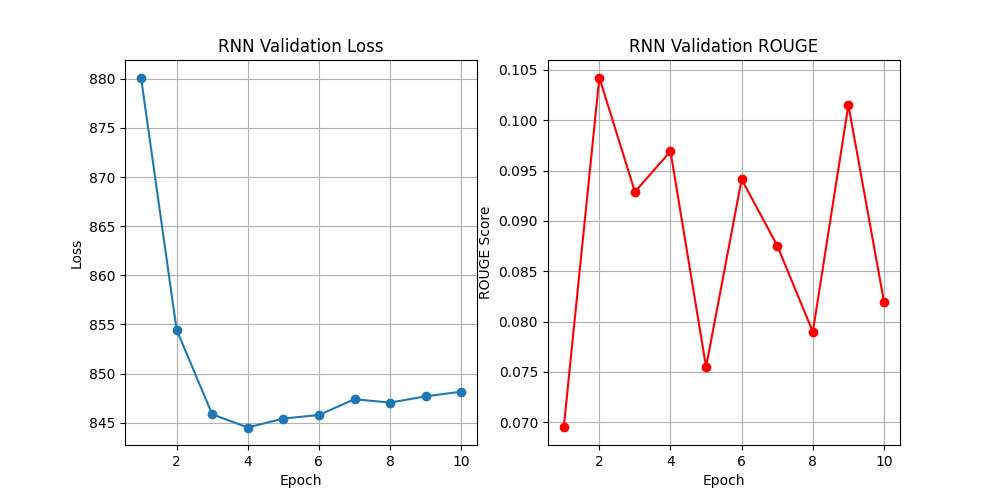
\includegraphics[width=0.5\textwidth,valign=c]{RNNResult.png}} \\
  \hline
  LSTM & \raisebox{-\height}{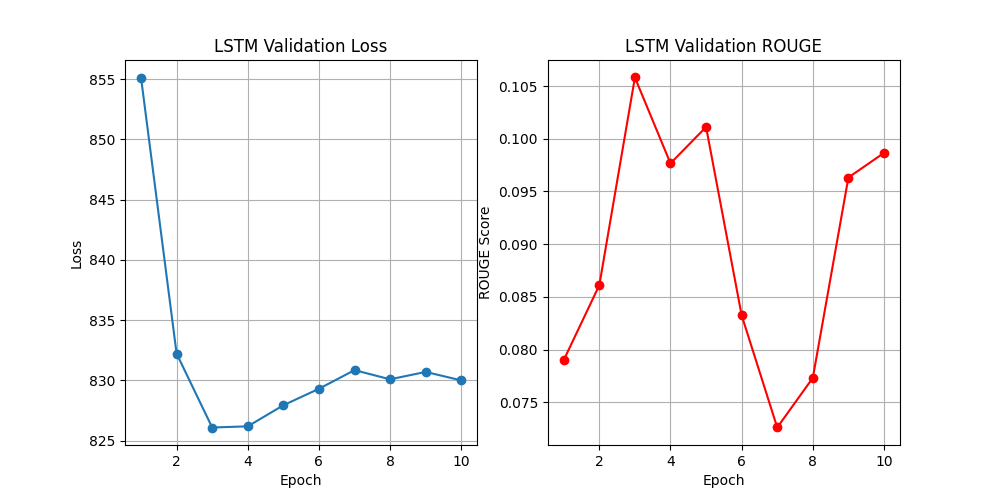
\includegraphics[width=0.5\textwidth,valign=c]{LSTMResult.png}} \\
  \hline
  GRU & \raisebox{-\height}{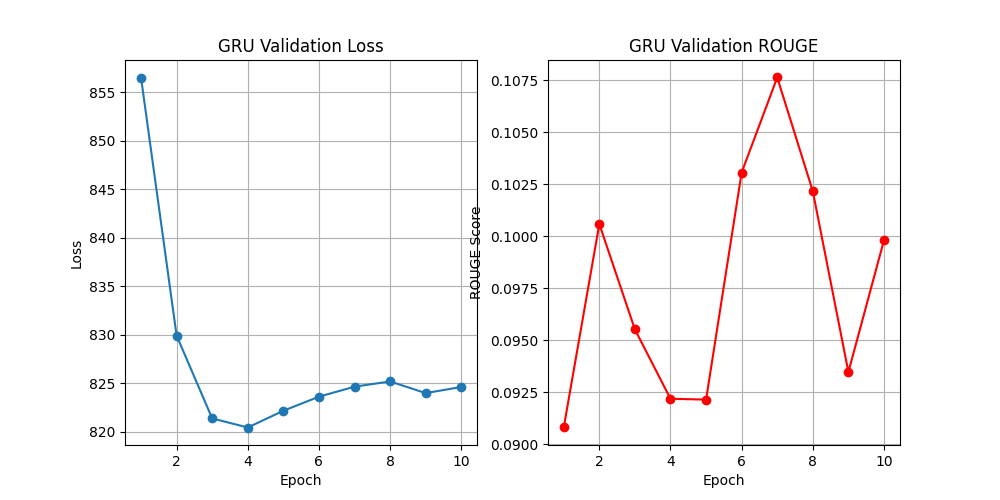
\includegraphics[width=0.5\textwidth,valign=c]{GRUResult.png}} \\
  \hline
\end{longtable}

\subsubsection{结果分析}
实际上这几个模型的结果都差不多,也都不够理想。在使用随机梯度下降的前提下,模型的均方误差都能不断降低并最终稳定在某个值,但ROUGE值却始终稳定在一个非常低的水平(大概$0.09$左右)。实验中也不是没有尝试过其他的超参数,但如果使用其他超参数,得到的结果只会更差。比如,如果把学习率的数量级调得更小或者更大,那模型的验证损失很早就不再下降了(甚至还会出现不降反增的情况);如果我们使用Adam优化器或者交叉熵损失,模型的ROUGE值会降低到$0.04$。究其原因,可能还是因为我们在把文本转化成向量的时候实际上是把已经脱敏变成向量的数据再转化成向量了一次,相当于对原始文本作了两次向量化,而且计算ROUGE指标的时候相当于还是用向量去作为输入计算指标的,但ROUGE指标需要使用原始文本作为输入。如果我们处理的就是原始文本,那么或许能够对模型作出更准确的评价。

\section{总结}
在本次实验中,我们使用深度学习开源软件搭建了三个可用于文本摘要的循环神经网络并测试了它们的性能,进一步体会到了神经网络的强大功能。

\end{document}